\newpage
\section{Qt-Framework Anwendung}

\subsection{Model-View Konzept}

In der Praxis werden viele User Interfaces mit dem MVC Pattern realisiert. Dieses Pattern besteht aus der View, dem Controller und dem Model. In diesem Zusammenhang wird eine strikte Trennung der einzelnen Schichten angestrebt. Das Ziel dieses Ansatzes, liegt in dem Austausch der View, ohne eine Anpassung der internen Datenstruktur durchführen zu müssen. Eine weitere Variante dieses Konzeptes ist das Model/View Konzept. Hierbei wird die View mit dem Controller kombiniert. Die Aufgabe der View es ist mit Hilfe des Models dem Benutzer die Informationen anzuzeigen. Der Controller reagiert lediglich auf Interaktion des Benutzers mit der View. Zusätzlich kann bei einer Model/View Architektur das Konzept eines „delegates“ eingeführt werden. Dieser besitzt die Aufgabe, die einzelnen Datenelemente des Models benutzerspezifisch anzuzeigen oder auf bestimmte Veränderungen des Datenbestandes von Seiten des Benutzers auf der View zu reagieren. Das Zusammenspiel der einzelnen Komponenten wird in Abbildung 1 nochmals graphisch veranschaulicht. \\

\begin{center}
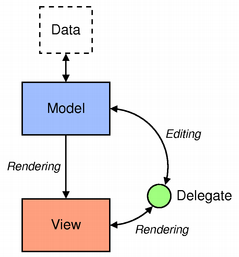
\includegraphics[scale=1.0]{images/ModelView.png}  \\
\end{center}

In Abbildung 1 wird deutlich, dass eine Trennung zwischen der Speicherung und der Darstellung der Daten besteht. Die Aufgabe des Models besteht darin, der View und dem Delegate minimalistische Schnittstellen für die Kommunikation bereitzustellen. Die Kommunikation zwischen den einzelnen Komponenten wird in QT mit Hilfe des Signal und Slot Konzeptes realisiert. Findet eine Änderung am Datenbestand des Models statt, wird ein Signal an die View und den entsprechenden Delegate geschickt. Diese rufen die entsprechenden Slots auf und aktualisieren die View. Im umgekehrten Fall, wenn der Benutzer die Daten via View verändert, schickt diese ein Signal an das Model und den Delegate. Ein weiteres Hilfsmittel der View ist der Modelindex. Dieser Index wird verwendet, um die einzelnen Informationen aus dem Datenbestand zu lesen. \\

Ein Modelindex ist eine Referenz auf einen einzelnen Datensatz des Models. Durch die Zuhilfenahme eines Delegates, kann dieser benutzerspezifisch auf der View dargestellt werden. Diesbezüglich muss erwähnt werden, dass es mehrere Möglichkeiten für die Erstellung der View unter QT existieren. Eine Möglichkeit ist die Erstellung mittels QT Widgets. Diese können durch Qt bereitgestellte Klassen erzeugt werden. Hierbei ist eine eindeutige Trennung zwischen View und Model schwer möglich. Eine andere Variante ist die Erstellung mittels QML. QML ist eine Art Beschreibungssprache für Benutzeroberflächen. Hierbei muss lediglich eine Beschreibung der GUI angegeben werden. Diese ist so allgemein gehalten, dass Designer oder UI-Entwickler ohne irgendwelche Vorkenntnisse einer Programmiersprache eine View anfertigen können. Der Vorteil hiervon liegt in der klaren Trennung der einzelnen Aufgaben. Ein Designer kann sich ausschließlich um das UI kümmern und ein Software-Entwickler um das dazugehörige Model und den Controller. Diesbezüglich existiert eine klare Trennung zwischen dem Model und der View.\\

In Qt sind alle Model Klassen von der Abstrakten Basisklasse QAbstractItemModel abgeleitet. Diese Basisklasse bietet eine Vielzahl an Schnittstellen für die Kommunikationen mit der View an. Um auf eine gegeben Datenstruktur besser reagieren zu können, bietet QT 3 besondere Model-Typen an. Diese Modeltypen sind: QListModel, QTableModel und QTreeModel. Mit Hilfe dieser 3 Modeltypen, kann eine Vielzahl der Anwendungsbereiche abgedeckt werden. In diesem Projekt ist ausschließlich ein QAbstractListModel verwendet worden. Zur Umsetzung des Model View/Konzeptes wurde für die Bereitstellung der UI die Beschreibungssprache QML verwendet. Für die Implementierung des Models wurde die bereits von Qt bereitgestellte Klasse QAbstractListModel verwendet. Hierbei ist eine neue Unterklasse von QAbstractListModel erzeugt und die entsprechenden Methoden für die Kommunikation mit der View neu implementiert worden. Als Datenstruktur wurde eine QList mit entsprechenden Datenobjekten gewählt. Die Datenobjekte besitzen die Aufgabe, die einzelnen Messwerte einer Messung zu kapseln. Eine Vielzahl der QML Elemente wie beispielsweise eine ListView oder TableView bieten standartmäßig eine Property „model“ an, welche die Verknüpfung mit dem entsprechenden Model realisiert. Des Weiteren kann mittels QML ein delegate Objekt erzeugt werden. Mit dessen Hilfe, können beispielsweise die Einträge in einer ListView bestmöglich auf die Wünsche des End-Benutzers angepasst werden. \\

Der Vorteil des QT Frameworks ist die automatische Anpassung der GUI an eine Änderung des internen Datenbestandes. Der Entwickler muss lediglich dem Model mitteilen, wann eine Änderung am Datenbestand des Models durchgeführt wurde. Infolgedessen übernimmt das Framework die komplette Aktualisierung der GUI. Der umgekehrte Fall, dass der Benutzer die Daten mittels GUI verändern kann, ist im Projektverlauf nicht implementiert worden. \\

Für die bestmögliche Darstellung der gesammelten Daten, mussten mehrere Diagramme erstellt werden. Hierbei bestand die Möglichkeit, alle Diagramme über die von QT bereitgestellten Klassen zu erzeugen, oder ein bereits vorhandenes auf QT basierendes Modul namens QCustomPlot zu verwenden. Dieses Modul kapselt die von QT bereitgestellten „Paint“ Klassen und gibt dem Benutzer eine Vielzahl an bereits vorimplementierten Diagramm-Typen. Ursprünglich wurde diese Third-Party Modul für den Einsatz mit QT Widgets konzipiert. Diesbezüglich musste eine Portierung in QML durchgeführt werden. Folglich konnten einige Funktionalitäten wie beispielsweise das Zoomen nicht in QML überführt werden. Die Portierung ist mittels der QCustomPlot Support Seite durchgeführt worden. \\

TODO: Quellen einfügen
Quellen:

http://qt-project.org/doc/qt-4.8/modelview.html

http://qt-project.org/doc/qt-4.8/model-view-programming.html

http://sysmagazine.com/posts/181712/

http://doc.qt.io/qt-5/qtqml-cppintegration-interactqmlfromcpp.html

http://qt-project.org/doc/qt-4.8/qmlevents.html

http://qt-project.org/doc/qt-4.8/qtbinding.html\#exchanging-data-between-qml-and-c

http://www.qcustomplot.com/index.php/support/forum/172

http://www.qcustomplot.com/index.php/tutorials/settingup

The Book of QT 4.0 Daniel Molkentin


\subsection{Umsetzung mittels QML}

Die Qt-Meta-Language kurz QML ist eine deklarative Programmiersprache für die Erstellung von Benutzeroberflächen. QML ist ein Teil von QtQuick und stellt eine Alternative zum Qt-Widget System dar. Die Hauptintention von QML ist die Erstellung von Benutzeroberflächen für Mobile-Systeme oder Desktop-Anwendungen. Hierfür ist eine einfache Syntax gewählt worden, sowie eine Integration von externem JavaScript Code. Infolgedessen, kann eine Trennung der Back-End und Front-End Entwicklung einer Applikation realisiert werden. Dieser Umstand zeigt einen großen Vorteil von QML gegenüber dem Qt-Widget System. Das Qt-Widget System, ermöglicht die Erstellung von Benutzeroberflächen mit Hilfe von C++ Code. Der Nachteil hiervon ist zum einen die fehlende Trennung von Applikation und Darstellungsschicht und zum anderen die mangelnde Übersicht im Quellcode bezüglich der View. Darüberhinaus ermöglicht QML die Erstellung von Animationen ohne zusätzliche Hilfsmittel. Des Weiteren können 3D- Animationen mittels OpenGl performanter und weniger fehleranfälliger als beim Qt-Widget System gezeichnet werden. \\

Durch die Verwendung von QML wird dem Entwickler eine Vielzahl an Freiheiten angeboten. Diese können beispielsweise für die Erstellung von eigenen Komponenten oder die benutzerdefinierte Anpassung von standardisierten Elementen genutzt werden. Im Verlauf des Projektes, sind mehrere QML Elemente benutzerspezifisch angepasst worden. Im Nachfolgenden wird eine QML spezifische Technik vorgestellt, wie ein QML Element durch den Entwickler manuell angepasst werden kann. \\

Für die Realisierung eines eigenen benutzerspezifischen QML Elements bietet QML  eine Property namens „style“ an. Mit Hilfe dieser, kann die Standardimplementierung eines QML Elements überschrieben werden. In Abbildung XX ist ein einfaches Tab Element mit Hilfe einer TabViewStyle, sowie einer neuen Tab-Komponente benutzerspezifisch angepasst worden. \\

\begin{center}
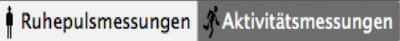
\includegraphics[scale=0.5]{images/TabView.png}  \\
\end{center}


Hierfür ist zu Beginn eine neue QML-Datei mit dem Namen der neuen Tab-Komponenten angelegt worden. Anschließend wurde der „style“ Property der TabView Komponente, welche die einzelnen Tab-Elemente zusammenfasst, ein neues TabViewStyle Element zugewiesen. Dieses Element enthält alle spezifischen Anpassungen bezüglich des angepassten Tabs. In diesem Fall ist die Farbe, Größe, Schrift, Höhe bzw. Breite des Standard Tabs angepasst worden. Ebenfalls ist ein neues Icon dem Tab hinzugefügt worden, um dem Anwender einen besseren Überblick auf die Applikation zu geben. \\

Abschließend sollte noch erwähnt werden, dass die Third-Party Komponente QCostumPlot (Erstellung der Diagramme) mit Hilfe einer eigenen QML Komponenten in die bestehende View integriert wurde. Hierfür musste ein neuer QML Type registriert und an der View angemeldet werden. Zusätzlich wurde das QML State System für das Aktualisieren der einzelnen Diagramme verwendet.

\subsection{Datenübertragung}
\subsubsection{Verzicht auf Bluetooth}
Ursprünglich war geplant die Datenübertragung vom Smartphone zur Desktop-PC-Anwendung mittels Serial-Port-Profile oder RFCOMM über Bluetooth zu implementieren. Allerdings zeigte sich sehr früh beim Implementierungsversuch mittels der Qt-Bluetooth Klassen-Bibliothek QBluetooth einige Schwierigkeiten bezüglich der Plattformunabhängigkeit. QBluetooth unterstützt lediglich Mac, Linux und Android. Windows wird aufgrund seiner Vielzahl uneinheitlicher Bluetooth-Stacks nicht unterstützt. Da zu erwarten ist, dass der Großteil der Zielgruppe von HeartRate2Go Windows als Betriebssystem einsetzt, wurde die Alternative TCP/IP gewählt.

\subsubsection{TCP-Server}
Die Qt-Komponente der HeartRate2Go Anwendung agiert für die Datenübertragung als TCP-Server. Die Umsetzung wird mit Hilfe der QTcpServer-Klasse der Qt-Bibliothek vorgenommen\cite{qtcpserver}. Eingehende Verbindungen werden in der TcpConnection-Klasse verarbeitet, die sich von der QThread-Klasse ableitet und dadurch die asynchrone Verarbeitung mehrerer Verbindungen sicherstellt.\\
\\
Wenn der TcpServer eine eingehende Verbindung annimmt, erzeugt er ein Objekt der TcpConnection-Klasse und übergibt ihr den Connection-Socket. Anschließend erhält der Thread des TcpConnection-Objekts die Kontrolle über diese Verbindung.\\
\\
Die Thread-Loop der TcpConnection-Klasse wartet auf eingehende Bytes und hängt diese an ein QByteArray-Objekt an. Nach dem Trennen der Verbindung wird dieses QByteArray zur weiteren Auswertung an den DataReceiver übergeben.

\subsubsection{Server-Discovery}
Um bei der Verwendung einer TCP/IP-Datenübertragung eine sichere Konnektivität zwischen Smartphone und Desktop-PC zu gewährleisten, muss der Anwender einen zusätzlichen Konfigurationsaufwand zur Ermittlung und Konfiguration der IP-Adresse in Kauf nehmen. Die HeartRate2Go Desktop-Anwendung verfügt deshalb über einen UDP-Server, der mittels eines einfachen Broadcast-Protokolls die Server-Discovery automatisiert und so dem Anwender den Konfigurationsaufwand gänzlich erspart\footnote{Für Netze in denen Broadcast-Messages blockiert, oder über Netz-Grenzen hinweg geroutet werden, ist weiterhin eine manuelle Konfiguration notwendig.}.\\
\\
Die Implementierung des UDP-Servers in der BroadcastReceiver-Klasse erfolgt durch Ableitung von QThread und einem auf Port 45454 gebundenen QUdpSocket-Objekt\cite{qudpsocket}. Die Thread-Loop wartet anschließend auf eingehende Datagramme.\\
\\
Beim Eintreffen eines Datagramms wird zunächst überprüft, ob es sich dabei um das erwartete Magic-Packet handelt. Ist dies der Fall, wird das Datagramm an den Absender an Port 45455 zurück gesendet. Der ursprüngliche Absender kann dadurch beim Empfang der Antwort die IP-Adresse des Servers ermitteln und eine TCP-Verbindung herstellen. Hat sich das Magic-Packet als falsch herausgestellt, wird das Datagramm verworfen.\\
\\
Bei dem Magic-Packet handelt es sich um den ASCII-String der UUID ''86417ce4-4f19-4a59-ae27-f404653e9751''.

\subsubsection{DataReceiver}
Die DataReceiver-Klasse nimmt das eigentliche Parsing des vom Smartphone erhaltenen Byte-Vektors unter Beachtung der Network-Byte-Order vor. Sie abstrahiert lediglich die Byte-Vektor-Darstellung der Daten von der vom Modell benötigten Listen-Repräsentation. Die Klasse ist als Singleton implementiert, da sie aufgrund des verwendeten Signal-Slot-Konzepts instanziiert werden muss.\\
\\
Der Parsevorgang wird mit Hilfe eines Zustandsautomaten realisiert, da die zu erwartenden Daten einem festgelegten Schema folgen müssen.\\
\\
Nach einem erfolgreichen Parsevorgang werden die so gewonnenen Datensätze an die ImportExport-Klasse übermittelt und der FilterController mit einem Signal über das Eintreffen neuer Daten benachrichtigt.\\
\\
In den Tabellen \ref{tbl:pdu} und \ref{tbl:datafield-description} wird das für die Datenübertragung verwendete Protokoll erläutert. Das \textit{Data}-Datenfeld darf dabei als einziges Datenfeld mehrfach vorkommen und dient zur Übertragung der einzelnen vorgenommenen Messungen während eines Gesamt-Messvorgangs. Bei einer Ruhemessung ist hier ein einziger Datensatz zu erwarten. Bei einer Aktivitätsmessung ist die Anzahl der \textit{Data}-Datensätze abhängig von der Dauer der Messung und des konfigurierten Messintervalls. Weiterhin dient ein leeres \textit{Data}-Feld als Sentinel um das korrekte Ende der Übertragung (EOT) zu signalisieren.
\begin{table*}[h]
	\centering
		\begin{tabularx}{\textwidth}{l|l|l|X}
			\hline
			Bezeichnung & Byte & Länge & Beschreibung \\
			\hline
			\hline
			Mode & \texttt{0x00} & 1 & Typ der Messung\\
			\hline
			Mood & \texttt{0x01} & 1 & Gemütszustand bei der Messung\\
			\hline
			Average & \texttt{0x02} & 2 & Durchschnitt aller Messwerte\\
			\hline
			Data & \texttt{0xff} & 12/0 & Datensatz eines Messpunktes/EOT\\
			\hline
		\end{tabularx}
		\caption{Protokoll-Datenfelder der Datenübertragung (Länge in Byte)}
		\label{tbl:pdu}
\end{table*}

\begin{table*}[h]
	\centering
		\begin{tabularx}{\textwidth}{l|l|l|X}
			\hline
			Bezeichnung & Länge & Typ & Beschreibung \\
			\hline
			\hline
			Zeitstempel & 8 & ulong & Zeitpunkt in Millisekunden des aktuellen Messpunktes\\
			\hline
			Puls & 2 & ushort & Pulswert dieses Messpunktes\\
			\hline
			Schritte & 2 & ushort & Anzahl der Schritte (inkrementell)\\
			\hline
		\end{tabularx}
		\caption{Aufbau des \textit{Data}-Datenfeldes aus Tabelle \ref{tbl:pdu}}
		\label{tbl:datafield-description}
\end{table*}

\subsection{Datenhaltung}
\subsubsection{SQLite}
Zur Speicherung sämtlicher Messungen, und damit verbundenen Datensätzen, wird auf die SQLite-Datenbankengine zurückgegriffen. Das Qt-Framework bietet mit der QSqlDatabase-Klasse eine Abstraktion zu vielen SQL-basierenden Datenbankengines an\cite{qsqldatabase}. Unter anderem unterstützt sie die SQLite-Engine. Der SQLite-Datenbank-Container wird plattformunabhängig im Benutzerverzeichnis des die Anwendung ausführenden Benutzers im Verzeichnis ''HeartRate'' gespeichert.

\subsubsection{Datenbankschema}
Das Datenbankschema besteht aus den vier in Abbildung \ref{pic:database-scheme} dargestellten Entitäten \textit{Measurement}, \textit{Data}, \textit{Mood} und \textit{Type}. 
\begin{figure}[H]
	\centering
	\visioToPDF{images/database-schema.pdf}
	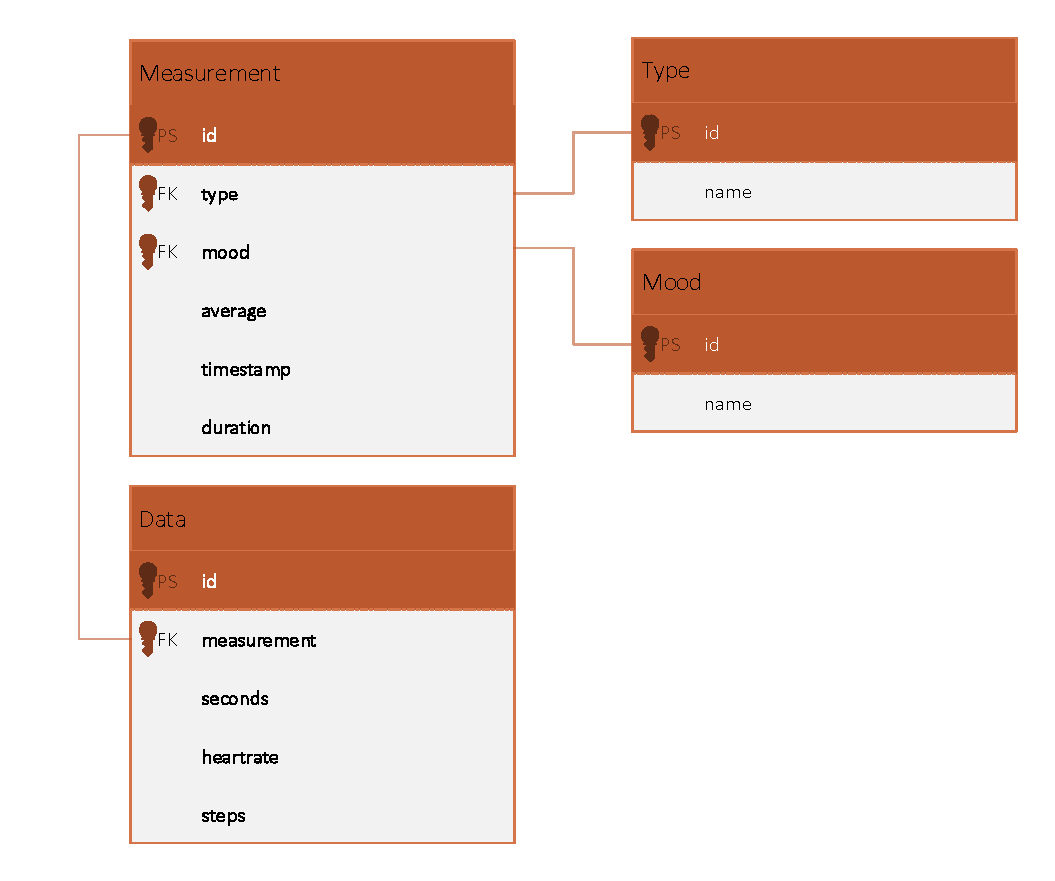
\includegraphics[width=0.9\textwidth]{images/database-schema.pdf}
	\caption{Das SQLite Datenbankschema}
	\label{pic:database-scheme}
\end{figure}

Tabelle \ref{tbl:database-entities} erläutert deren Aufgaben im Einzelnen.
\begin{table*}[h]
	\centering
		\begin{tabularx}{\textwidth}{l|X}
			\hline
			DB-Tabelle & Beschreibung \\
			\hline
			\hline
			Measurement & Speichert allgemeine Informationen \textbf{einer} Messung\\
			\hline
			Data & Speichert die einzelnen Messwerte zu einem \textit{Measurement}-Eintrag\\
			\hline
			Mood & Speichert die möglichen Gefühlszustände, die jeder Messung zugeordnet werden\\
			\hline
			Type & Speichert die möglichen Messungstypen, die jeder Messung zugeordnet werden\\
			\hline
		\end{tabularx}
		\caption{Aufbau des \textit{Data}-Datenfeldes aus Tabelle \ref{tbl:pdu}}
		\label{tbl:database-entities}
\end{table*}
